%!TEX root = ../../book_ML.tex
\chapter{Các kỹ thuật xây dựng đặc trưng}
\label{cha:feature} 
 
\section{Giới thiệu }
 
% Cho tới lúc này, tôi đã trình bày 5 thuật toán Machine Learning cơ bản: \href{http://machinelearningcoban.com/2016/12/28/linearregression/}{Linear Regression}, \href{http://machinelearningcoban.com/2017/01/01/kmeans/}{$K$-means Clusterning}, \href{http://machinelearningcoban.com/2017/01/08/knn/}{K-nearest neighbors}, \href{http://machinelearningcoban.com/2017/01/21/perceptron/}{Perceptron Learning Algorithm} và \href{http://machinelearningcoban.com/2017/01/27/logisticregression/}{Logistic Regression}. Trong tất cả các thuật toán này, tôi đều giả sử các điểm dữ liệu được biểu diễn bằng các vector, được gọi là \textit{feature vector} hay \textit{vector đặc trưng}, có độ dài bằng nhau, và cùng là vector cột hoặc vector hàng. Tuy nhiên, trong các bài toán thực tế, mọi chuyện không được tốt đẹp như vậy! 

% \index{feature engineering}
\index{vector đặc trưng -- feature vector}
Mỗi điểm dữ liệu trong một mô hình machine learning thường được biểu diễn bằng
một vector được gọi là \textit{vector đặc trưng} (feature vector). Trong cùng một mô hình, các
vector đặc trưng của các điểm thường có kích thước như nhau. Điều này là cần
thiết vì các mô hình bao gồm các phép toán với ma trận và vector, các phép toán
này yêu cầu dữ liệu có chiều phù hợp. Tuy nhiên, dữ liệu thực tế thường ở dạng
thô với kích thước khác nhau hoặc kích thước như nhau nhưng số chiều quá lớn gây
trở ngại trong việc lưu trữ. Vì vậy, việc lựa chọn, tính toán đặc trưng phù hợp
cho mỗi bài toán là một bước quan trọng.

Trong những bài toán {thị giác máy tính}, các bức ảnh thường là các ma trận hoặc
mảng nhiều chiều với kích thước khác nhau. Các bức ảnh này có thể được chụp bởi nhiều camera trong các điều kiện ánh sáng khác nhau. Các bức ảnh này không những cần được đưa về kích thước phù hợp mà còn cần được chuẩn hoá để tăng hiệu quả của mô hình. 


% Trong bài toán nhận dạng vật thể
% trong ảnh, đôi khi ta cần làm thêm một bước nữa là \textit{xác định vị trí vật
% thể}, bao gồm  tức là tìm các khung chứa vật thể cần dự đoán.
% Ví dụ, trong bài toán nhận dạng khuôn mặt, ta cần tìm được vị trí các khuôn mặt
% trong ảnh và cắt ra các khuôn mặt đó trước khi làm các bước tiếp theo. Ngay cả
% khi đã xác định được các khung chứa các khuôn mặt, ta vẫn phải làm rất nhiều
% việc vì hình ảnh của khuôn mặt còn phụ thuộc vào góc chụp, ánh sáng,... và rất
% nhiều yếu tố khác nữa.
Trong các bài toán xử lý ngôn ngữ tự nhiên, độ dài văn bản có thể khác nhau, được viết theo những văn phong khác nhau. Trong nhiều trường hợp, việc thêm bớt một vài từ vào một văn bản có thể thay đổi hoàn toàn nội dung của nó. Hoặc
cùng là một câu nói nhưng tốc độ, âm giọng của mỗi người là khác nhau, tại
các thời điểm khác nhau là khác nhau. 
% thậm chí
% của cùng một người nhưng lúc ốm lúc khỏe cũng khác nhau.
\index{trích chọn đặc trưng -- feature extraction}
Khi làm việc với các bài toán machine learning, nhìn chung ta chỉ có được dữ
liệu thô chưa qua chỉnh sửa và chọn lọc. Ngoài ra, ta có thể phải loại bỏ những
dữ liệu nhiễu và đưa dữ liệu thô với kích thước khác nhau về cùng một chuẩn. Dữ
liệu chuẩn này phải đảm bảo giữ được những thông tin đặc trưng của dữ liệu
thô ban đầu. Không những thế, ta cần thiết kế những phép
biến đổi để có những đặc trưng phù hợp cho từng bài toán. Quá trình quan trọng này được gọi là \textit{trích chọn đặc trưng} ({feature extraction} hoặc {feature engineering}).

% Xin trích một câu nói (xin không dịch) của Andrew Ng\footnote{
% \textit{Feature Engineering --  Wikipedia} (\url{https://goo.gl/v4e21T})}:
 
% \textit{Coming up with features is difficult, time-consuming, requires expert
% knowledge. ``Applied machine learning'' is basically feature engineering.}

Để có cái nhìn tổng quan, chúng ta cần đặt bước trích chọn đặc trưng này trong cả quy trình xây dựng một mô hình machine learning.
 
 
\section{Mô hình chung cho các bài toán machine learning }
% ******************************************************************************
\begin{figure}[t]
\centering
    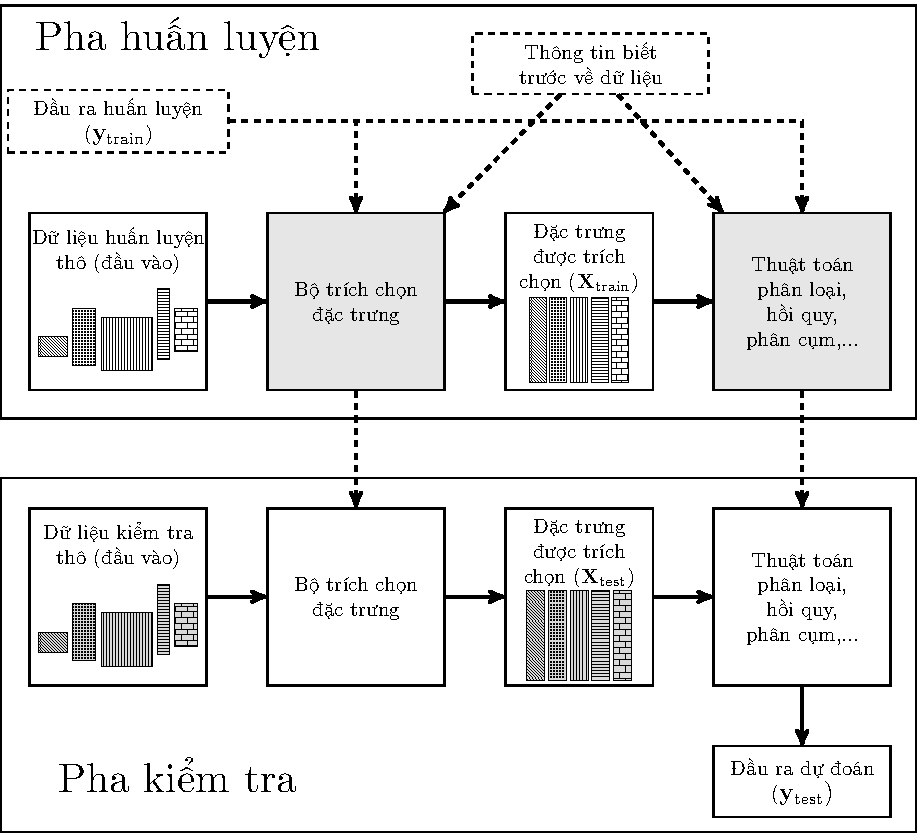
\includegraphics[width = \textwidth]{Chapters/01_Overview/11_featureengineering/latex/ML_models2.pdf}
    \caption[]{Mô hình chung trong các bài toán machine learning}
    \label{fig:11_1}
\end{figure}
% ******************************************************************************


% Với các bài toán supervised learning, ta có các cặp dữ liệu (\textit{input,
% output}), với các bài toán unsupervised learing, ta chỉ có \textit{input}. Khi
% thực hiện một thuật toán machine learning, toàn bộ dữ liệu có được thường được
% chia làm hai tập hợp không giao nhau: tập huấn luyện và tập kiểm thử. Với các
% thuật toán supervised learning, khi phân chia, ta cần chú ý phân chia đúng các
% cặp (\textit{input}, \textit{output}) của dữ liệu. 

Phần lớn các mô hình machine learning có thể được minh hoạ trong
Hình~\ref{fig:11_1}. Có hai pha lớn trong mỗi bài toán machine learning là
\textit{pha huấn luyện} (training phase) và \textit{pha kiểm tra} (test phase). Pha huấn luyện xây dựng mô
hình dựa trên dữ liệu huấn luyện. Dữ liệu kiểm tra được sử dụng để đánh giá
hiệu quả mô hình\footnote{Trước khi đánh giá một mô hình trên tập kiểm tra, ta
cần đảm bảo rằng mô hình đó đã làm việc tốt trên tập huấn luyện.}.

\subsection{Pha huấn luyện}
Có hai khối có nền màu xám cần được thiết kế:  

Khối trích chọn đặc trưng có nhiệm vụ tạo ra một
vector đặc trưng cho mỗi điểm dữ liệu đầu vào. Vector đặc trưng này thường có
kích thước như nhau, bất kể dữ liệu đầu vào có kích thước như thế nào.

Đầu vào của khối trích chọn đặc trưng có thể là các yếu tố sau: 

\begin{itemize}
    \item \textit{Dữ liệu huấn luyện đầu vào ở dạng thô} bao gồm tất cả các thông tin ban đầu. Ví dụ, dữ liệu thô của một ảnh là
    giá trị của từng điểm ảnh, của một văn bản là từng từ, từng câu; của một
    file âm thanh là một đoạn tín hiệu; của thời tiết là thông tin về hướng gió,
    nhiệt độ, độ ẩm không khí,... Dữ liệu thô này thường không ở dạng vector,
    không có số chiều như nhau hoặc một vài thông tin bị khuyết. Thậm chí chúng
    có thể có số chiều như nhau nhưng rất lớn. Chẳng hạn, một bức ảnh màu kích
    thước $1000\times 1000$ có số điểm ảnh là $3 \times 10^6$\footnote{Ảnh màu
    thường có ba kênh: red, green, blue -- RGB}. Đây là một con số quá lớn, không có lợi cho lưu
    trữ và tính toán.

    \item \textit{Dữ liệu huấn luyện đầu ra}: dữ liệu này có thể được sử dụng
    hoặc không. Trong các thuật toán học không giám sát, ta không biết đầu ra
    nên hiển nhiên không có giá trị này. Trong các thuật toán học có giám sát,
    đôi khi dữ liệu này cũng không được sử dụng. Ví dụ, việc giảm chiều dữ liệu
    có thể không cần sử dụng dữ liệu đầu ra. Nếu dữ liệu đầu vào đã là các
    vector cột cùng chiều, ta chỉ cần nhân vào bên phải của chúng một ma trận
    chiếu ngẫu nhiên. Ma trận này có số hàng ít hơn số cột để đảm bảo số chiều
    thu được nhỏ hơn số chiều ban đầu. Việc làm này mặc dù làm mất đi thông tin,
    trong nhiều trường hợp vẫn mang lại hiệu quả vì đã giảm được lượng tính toán
    ở phần sau. Đôi khi {ma trận chiếu} không phải là ngẫu nhiên mà có thể được
    \textit{học} dựa trên toàn bộ dữ liệu thô ban đầu (xem Chương~\ref{cha:pca}).

    Trong nhiều trường hợp khác, dữ liệu đầu ra của tập huấn luyện cũng được sử
    dụng để tạo bộ trích chọn đặc trưng. Việc giữ lại
    nhiều thông tin không quan trọng bằng việc giữ lại các thông tin có ích. Ví dụ, dữ liệu thô là các hình vuông và hình tam giác màu đỏ và xanh.
    Trong bài toán phân loại đa giác, nếu các nhãn là \textit{tam giác} và
    \textit{vuông}, ta không quan tâm tới màu sắc mà chỉ quan tâm tới số cạnh
    của đa giác. Ngược lại, trong bài toán phân loại màu với các nhãn là
    \textit{xanh} và \textit{đỏ}, ta không quan tâm tới số cạnh mà chỉ quan tâm
    đến màu sắc.

    \item \textit{Các thông tin biết trước về dữ liệu}: Ngoài dữ liệu huấn luyện, các thông tin biết trước ngoài lề cũng có tác dụng trong việc xây dựng bộ trích chọn đặc trưng. Chẳng hạn, có thể dùng các bộ lọc để giảm nhiễu nếu dữ liệu là âm thanh, hoặc dùng các bộ dò cạnh để tìm ra cạnh của các vật thể trong dữ liệu ảnh. Nếu dữ liệu là ảnh các tế bào và ta cần đưa ảnh về kích thước nhỏ hơn, ta cần lưu ý về độ phân giải của tế bảo của ảnh trong kích thước mới. Ta cần xây dựng một bộ trích chọn đặc trưng phù hợp với từng loại dữ liệu. 
\end{itemize}

\index{dac@đặc trưng đã trích xuất -- extracted feature}
Sau khi xây dựng bộ trích chọn đặc trưng, dữ liệu thô ban đầu được đưa qua và
tạo ra các vector đặc trưng tương ứng gọi là \textit{đặc trưng đã trích
xuất} ({extracted feature}). Những đặc trưng này được dùng để huấn luyện
các thuật toán machine learning chính như phân loại, phân cụm, hồi quy,... trong
khối màu xám thứ hai.

% \index{state-of-the-art}
\index{end-to-end}
\newnote{}{
Trong một số thuật toán cao cấp hơn, việc xây dựng bộ trích chọn đặc trưng và
các thuật toán chính có thể được thực hiện đồng thời thay vì riêng lẻ như trên.
Đầu vào của toàn bộ mô hình là dữ liệu thô hoặc dữ liệu thô đã qua một bước xử
lý nhỏ. Các mô hình đó có tên gọi chung là `mô hình đầu cuối' (end-to-end
model). Với sự phát triển của deep learning trong những năm gần đây, người ta
cho rằng các mô hình đầu cuối mang lại kết quả tốt hơn nhờ vào việc hai khối
được huấn luyện cùng nhau, bổ trợ lẫn nhau cùng hướng tới mục đích chung cuối
cùng. Thực tế cho thấy, các mô hình machine learning hiệu quả nhất thường là các
mô hình đầu cuối. }

%     Khi xây dựng bộ \textit{feature extractor} và \textit{main algorithms},
%     chúng ta không được sử dụng bất kỳ thông tin nào trong tập \textit{test data}. Ta phải giả sử rằng những thông tin trong \textit{test data} chưa được nhìn thấy bao giờ. Nếu sử dụng thêm thông tin về \textit{test data} thì rõ ràng ta đã \textit{ăn gian}
% \end{mynote}

% \textbf{Một điểm rất quan trọng: khi xây dựng bộ \textit{feature extractor} và \textit{main algorithms}, chúng ta không được sử dụng bất kỳ thông tin nào trong tập \textit{test data}. Ta phải giả sử rằng những thông tin trong \textit{test data} chưa được nhìn thấy bao giờ. Nếu sử dụng thêm thông tin về \textit{test data} thì rõ ràng ta đã \textit{ăn gian}! Tôi từng đánh giá các bài báo khoa học quốc tế, rất nhiều tác giả xây dựng mô hình dùng cả dữ liệu \textit{test data}, sau đó lại dùng chính mô hình đó để kiểm tra trên \textit{test data} đó. Việc \textit{ăn gian} này là lỗi rất nặng và hiển nhiên những bài báo đó bị từ chối (reject).} 
 
 
\subsection{Pha kiểm tra}

Ở pha kiểm tra, vector đặc trưng của một điểm dữ liệu thô mới được tạo bởi bộ trích chọn đặc trưng thu được từ pha huấn luyện. Vector đặc trưng này được đưa
vào thuật toán chính đã tìm được để đưa ra quyết tra. Có một lưu ý quan trọng là khi xây dựng bộ trích chọn đặc trưng và các thuật toán chính, ta không được sử dụng dữ liệu kiểm tra. Các công việc đó được thực hiện chỉ dựa trên dữ liệu huấn luyện. 

% Bước này đơn giản hơn nhiều. Với \textit{raw input} mới, ta sử dụng feature
% extractor đã tạo được ở trên (tất nhiên không được sử dụng \textit{output} của nó vì \textit{output} là cái ta đang đi tìm) để tạo ra feature vector tương ứng. Feature vector được đưa vào \textit{main algorithm} đã được học ở training phase để dự đoán \textit{output}.
 
 
\section{Một số kỹ thuật trích chọn đặc trưng}
 
\subsection{Trực tiếp lấy dữ liệu thô}
% Với bài toán phân loại chữ số viết tay trong bộ cơ sở dữ liệu \href{http://machinelearningcoban.com/2017/01/04/kmeans2/#bo-co-so-du-lieu-mnist}{MNIST}, mỗi bức ảnh có số chiều là 28 điểm ảnh x 28 điểm ảnh (tất nhiên việc \textit{crop} và chỉnh sửa mỗi bức ảnh đã được thực hiện từ trước rồi, đó đã là một phần của feature engineering rồi). Một cách đơn giản thường được dùng là \textit{kéo dài} ma trận 28x28 này để được 1 vector có số chiều 784. Trong cách này, các cột (hoặc hàng) của ma trận ảnh được đặt chồng lên (hoặc cạnh nhau) để được 1 vector dài. Vector dài này được trực tiếp sử dụng làm feature đưa vào các bộ classifier/clustering/regression/... Lúc này, giá trị của mỗi điểm ảnh ảnh được coi là một feature.  

\index{vectorization -- vector hoá}
Xét bài toán với dữ liệu là các bức ảnh xám có kích thước cố tra $m\times n$
điểm ảnh. Cách đơn giản nhất để tạo ra vector đặc trưng cho bức ảnh này là xếp
chồng các cột của ma trận điểm ảnh để được một vector $m\times n$ phần tử.
Vector này có thể được coi là vector đặc trưng với mỗi đặc trưng là giá trị của
một điểm ảnh. Việc làm đơn giản này đã làm mất {thông tin về vị trí tương đối}
giữa các điểm ảnh vì các điểm ảnh gần nhau theo phương ngang trong bức ảnh ban
đầu không còn gần nhau trong vector đặc trưng. Tuy nhiên, trong
nhiều trường hợp, kỹ thuật này vẫn mang lại kết quả khả quan.
 
\subsection{Lựa chọn đặc trưng}
\index{lựa chọn đặc trưng -- feature selection}
Đôi khi, việc trích chọn đặc trưng đơn giản là chọn ra các thành phần phù hợp trong dữ liệu ban đầu. Việc làm này thường xuyên được áp dụng khi một lượng dữ liệu thu được không có đầy đủ các thành phần hoặc dữ liệu có quá nhiều chiều mà phần lớn không mang nhiều thông tin hữu ích. 
 
\subsection{Giảm chiều dữ liệu}
\index{giảm chiều dữ liệu -- dimensionality reduction}
% \index{chiếu ngẫu nhiên -- random projection}
\index{ma trận chiếu -- projection matrix}
\index{phân tích thành phần chính -- principal component analysis}
Giả sử dữ liệu ban đầu là một vector $\bx \in \R^D$, $\bA$ là một ma trận trong
$R^{d\times D}$ và $\bz = \bA\bx\in\R^d$. Nếu $d < D$, ta thu được một vector
với số chiều nhỏ hơn. Đây là một kỹ thuật phổ biến trong giảm chiều dữ liệu. Ma
trận $\bA$ được gọi là \textit{ma trận chiếu} (projection matrix), có thể là một ma trận ngẫu nhiên.
Tuy nhiên, việc chọn một ma trận chiếu ngẫu nhiên đôi khi mang lại kết quả tệ
không mong muốn vì thông tin có thể bị thất thoát quá nhiều. Một phương pháp phổ
biến để tối thiểu lượng thông tin mất đi có tên là \textit{phân tích thành phần
chính} ({principal component analysis}) sẽ được trình bày trong
Chương~\ref{cha:pca}.

\textit{Lưu ý:} {Kỹ thuật xây dựng đặc trưng không nhất thiết luôn làm giảm số
chiều dữ liệu, đôi khi vector đặc trưng có thể có có kích thước lớn hơn dữ liệu
thô ban đầu nếu việc này mang lại hiệu quả tốt hơn.}

% feature vector còn có số chiều lớn hơn raw data.
% Random projection
% cũng có thể làm được việc này nếu ma trận chiếu là một ma trận \textit{cao} (số
% cột ít hơn số hàng).
 
 
\subsection{Túi từ}
\index{túi từ -- bag of words}

Chúng ta hẳn đã tự đặt ra các câu hỏi: với một văn bản, vector đặc trưng sẽ có
dạng như thế nào? Làm sao đưa các từ, các câu, đoạn văn ở dạng ký tự
trong các văn bản về một vector mà mỗi phần tử là một số?
 
Có một kỹ thuật rất phổ biến trong xử lý văn bản có tên là \textit{túi từ}
({bag of words, BoW}).
 
Bắt đầu bằng ví dụ phân loại tin nhắn rác. Nhận thấy rằng nếu một tin có chứa
các từ {``khuyến mại'', ``giảm giá'', ``trúng thưởng'', ``miễn phí'', ``quà tặng'', ``tri
ân'',...}, nhiều khả năng đó là một tin nhắn rác. Từ đó, phương pháp đầu tiên có
thể nghĩ tới là {đếm} số lần các từ này xuất hiện, nếu số lượng này nhiều hơn
một ngưỡng nào đó thì ta quyết định đó là tin rác\footnote{Bài toán thực tế phức
tạp hơn khi các tin nhắn có thể được viết dưới dạng không dấu, bị cố tình viết
sai chính tả, hoặc dùng các ký tự đặc biệt}. Với các loại văn bản khác nhau,
lượng từ liên quan tới từng chủ đề cũng khác nhau. Từ đó có thể dựa vào số lượng
các từ trong từng loại để tạo các vector đặc trưng cho từng văn bản.
 
% Tôi xin lấy ví dụ cụ thể hơn về cách tạo ra vector đặc trưng cho mỗi văn bản dựa trên BoW và xin được lấy tiếng Anh làm ví dụ (nguồn \href{https://en.wikipedia.org/wiki/Bag-of-words_model}{Bag of Words wiki}. Tiếng Việt khó hơn vì một từ có thể có nhều âm tiết, tiếng Anh thì thường cứ gặp dấu cách là kết thúc một từ).  
% \newpage  
\index{túi từ -- bag of words!từ điển}
Xin lấy một ví dụ về hai văn bản đơn giản sau đây\footnote{\textit{Bag of
words -- Wikipedia} (\url{https://goo.gl/rBtZqx})}:
 
\begin{lstlisting}[language=Python]
(1) "John likes to watch movies. Mary likes movies too."
\end{lstlisting}
và   
\begin{lstlisting}[language=Python]
(2) "John also likes to watch football games." 
\end{lstlisting}
Dựa trên hai văn bản này, ta có danh sách các từ được sử dụng, được gọi là
\textit{từ điển} ({dictionary} hoặc {codebook}) với mười
\textit{từ} như sau:
 
\begin{lstlisting}[language=Python]
["John", "likes", "to", "watch", "movies", "also", "football", "games", "Mary", "too"] 
\end{lstlisting}
Với mỗi văn bản, ta sẽ tạo ra một vector đặc trưng có số chiều bằng 10, mỗi phần
tử đại diện cho số từ tương ứng xuất hiện trong văn bản đó. Với hai văn bản
trên, ta sẽ có hai vector đặc trưng:
\begin{lstlisting}[language=Python]
(1) [1, 2, 1, 1, 2, 0, 0, 0, 1, 1] 
(2) [1, 1, 1, 1, 0, 1, 1, 1, 0, 0] 
\end{lstlisting}
Văn bản (1) có một từ \pythoninline{"John"}, hai từ \pythoninline{"likes"}, không từ
\pythoninline{"also"}, không từ \pythoninline{"football"},... nên ta thu được
vector tương ứng như trên.
 
\index{vector thưa -- sparse vector}
Có một vài điều cần lưu ý trong BoW: 
\begin{itemize}
    \item Với những ứng dụng thực tế, {từ điển} có số lượng từ lớn hơn rất
    nhiều, có thể đến cả triệu, như vậy vector đặc trưng thu được sẽ rất dài.
    Một văn bản chỉ có một câu, và một tiểu thuyết nghìn trang đều được biểu
    diễn bằng các vector có kích thước như nhau.

    \item Có rất nhiều từ trong từ điển không xuất hiện trong một văn bản. Như
    vậy các vector đặc trưng thu được thường có nhiều phần tử bằng không.
    Các vector đó được gọi là \textit{vector thưa} (sparse vector). Để việc lưu trữ được hiệu quả hơn, ta không lưu mọi thành phần của một
    vector thưa mà chỉ lưu {vị trí} của các phần tử khác không và {giá
    trị} tương ứng. Chú ý rằng nếu có hơn một nửa số phần tử khác không, việc
    làm này lại phản tác dụng. Tuy nhiên, trường hợp này ít xảy ra vì hiếm có
    văn bản chứa tới một nửa số từ trong từ điển.

    \item Các từ hiếm gặp được xử lý như thế nào? Một kỹ thuật thường dùng là
    thêm phần tử \pythoninline{<Unknown>} vào trong từ điển. Mọi từ không có
    trong từ điển đều được coi là
    \pythoninline{<Unknown>}.

    \item Tuy nhiên, những từ hiếm đôi khi lại mang những thông tin quan
    trọng nhất mà chỉ loại văn bản đó có. Đây là một nhược điểm của BoW. Có một
    phương pháp cải tiến giúp khắc phục nhược điểm này tên là \textit{term
    frequency-inverse document frequency} (TF-IDF)~\cite{salton1975vector} dùng
    để xác định tầm quan trọng của một từ trong một văn bản dựa trên toàn bộ văn
    bản trong cơ sở dữ liệu\footnote{\textit{5 Algorithms Every Web Developer
    Can Use and Understand, section 5} (\url{https://goo.gl/LJW3H1}).}.

    \item Nhược điểm lớn nhất của BoW là nó không mang thông tin về thứ tự của
    các từ, cũng như sự liên kết giữa các câu, các đoạn văn trong văn bản. Thứ
    tự của các từ trong văn bản thường mang thông tin quan trọng. Ví dụ, ba câu
    sau đây: ``Em yêu anh không?'', ``Em không yêu anh'', và ``Không, (nhưng)
    anh yêu em'' khi được trích chọn đặc trưng bằng BoW sẽ cho ra ba vector
    giống hệt nhau, mặc dù ý nghĩa khác hẳn nhau.
\end{itemize}
 
% \textbf{Bonus:} hình dưới đay là tần suất sử dụng các từ (coi mỗi âm tiết là một từ) trong Truyện Kiều (\href{https://bitbucket.org/tiepvupsu/vietnamese/src/c6f3af6050f8ca911ed0fa209220ce3c99010075/TruyenKieu2.txt?at=master&fileviewer=file-view-default}{theo bản này}) nếu ta chỉ sử dụng 30 từ có tần suất cao nhất. : 
% <div class="imgcap"> 
% <img src ="\assets\FeatureEngineering\truyenkieu.png" align = "center" width = "400"> 
% <div class = "thecap">Hình 2: Bag of Words cho Truyện Kiều với 30 từ có tần suất cao nhất.</div> 
% </div>  
 
  
\subsection{BoW cho dữ liệu ảnh}
BoW cũng được áp dụng cho các bức ảnh với cách định nghĩa \textit{từ} và
\textit{từ điển} khác. Xét các ví dụ sau:
 
\textit{Ví dụ 1}: Giả sử có một tập dữ liệu ảnh có hai nhãn là rừng và sa mạc, và một bức ảnh chỉ rơi vào một trong hai loại này. Việc phân
loại một bức ảnh là rừng hay sa mạc một cách tự nhiên nhất là dựa vào màu sắc.
Màu xanh lục nhiều tương ứng với rừng, màu đỏ và vàng nhiều tương ứng với sa mạc. Ta có một mô hình đơn giản để trích chọn đặc trưng như sau:
\begin{itemize}
    \item Với một bức ảnh, chuẩn bị một vector $\mathbf{x}$ có số chiều bằng 3,
    đại diện cho ba màu xanh lục ($x_1$), đỏ ($x_2$), và vàng ($x_3$).  

    \item Với mỗi điểm ảnh trong bức ảnh đó, xem nó gần với màu xanh, đỏ hay
    vàng nhất dựa trên giá trị của điểm ảnh đó. Nếu nó gần điểm xanh nhất, tăng
    $x_1$ lên một; gần đỏ nhất, tăng $x_2$ lên một; gần vàng nhất, tăng $x_3$
    lên một.

    \item Sau khi xem xét tất cả các điểm ảnh, dù cho bức ảnh có kích thước thế
    nào, ta vẫn thu được một vector có kích thước bằng ba, mỗi phần tử thể hiện
    việc có bao nhiêu điểm ảnh trong bức ảnh có màu tương ứng. Vector cuối này còn
    được gọi là \textit{histogram vector} của bức ảnh và có thể coi là một vector đặc trưng tốt trong bài toán phân loại
    ảnh rừng hay say mạc. 
\end{itemize} 
  
\textit{Ví dụ 2}: Trên thực tế, các bài toán xử lý ảnh không đơn giản như trong
ví dụ trên đây. Mắt người thực ra nhạy với các đường nét, hình dáng hơn là màu
sắc. Chúng ta có thể nhận biết được một bức ảnh có cây hay không ngay cả khi bức
ảnh đó không có màu. Vì vậy, xem xét giá trị từng điểm ảnh không mang lại kết
quả khả quan vì lượng thông tin về đường nét đã bị mất.

\index{patch}
% ******************************************************************************
\begin{figure}[t]
\centering
    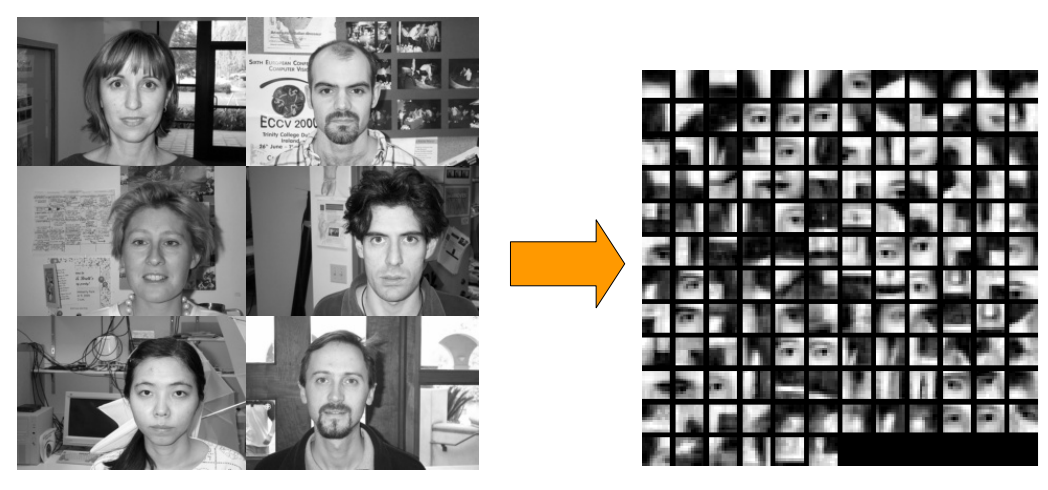
\includegraphics[width = \textwidth]{Chapters/01_Overview/11_featureengineering/bow_face.png}
    \caption[]{Bag of words cho ảnh chứa mặt người (Nguồn: \textit{Bag of
    visual words model: recognizing object categories}
    (\url{https://goo.gl/EN2oSM}).}
    \label{fig:11_2}
\end{figure}
% ******************************************************************************

Có một giải pháp là thay vì xem xét một điểm ảnh, ta xem xét một vùng hình chữ
nhật nhỏ trong ảnh, vùng này còn được gọi là \textit{patch}. Các patch này nên
đủ lớn để có thể chứa được các bộ phận đặc tả vật thể trong ảnh. Ví dụ với mặt
người, các patch cần chứa được các phần của khuôn mặt như mắt, mũi, miệng (xem
Hình~\ref{fig:11_2}). Tương tự, với ảnh là ô tô, các patch thu được có thể là
bánh xe, khung xe, cửa xe,...(xem Hình~\ref{fig:11_3}, hàng trên bên phải).
\begin{figure}[t]
\centering
    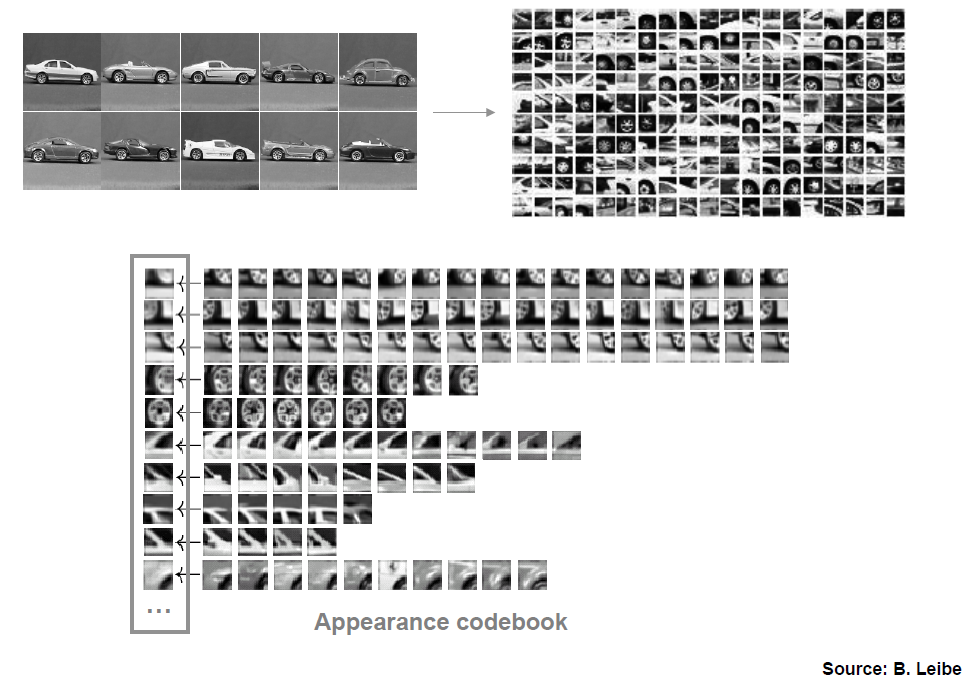
\includegraphics[width = \textwidth]{Chapters/01_Overview/11_featureengineering/bow_car.png}
    \caption[]{Bag of Words cho ảnh xe hơi (Nguồn: B. Leibe).}
    \label{fig:11_3}
\end{figure}
% <div class="imgcap"> 
% <img src ="\assets\FeatureEngineering\bow_car.png" align = "center" width = "800"> 
% <div class = "thecap">Hình 4: Bag of Words cho ảnh ô tô. (Nguồn: tôi cố gắng tìm nguồn cho hình này nhưng tất cả các tài liệu tôi tìm được đều ghi "Source: B. Leibe", tôi cũng xin được trích nguồn tương tự)</div> 
% </div>  
 
Trong xử lý văn bản, hai từ được coi là như nhau nếu nó được biểu diễn bởi các
ký tự giống nhau. Câu hỏi đặt ra là, trong xử lý ảnh, hai patch được coi là như
nhau khi nào? Khi mọi điểm ảnh trong hai patch có giá trị bằng nhau sao?
 
Câu trả lời là không. Xác suất để hai patch giống hệt nhau từng điểm ảnh là rất
thấp vì có thể một phần của vật thể trong một patch bị lệch đi, bị
méo, hoặc có độ sáng thay đổi. Trong những trường hợp này, mặc dù mắt người vẫn
thấy hai patch đó {rất giống nhau}, máy tính có thể nghĩ đó là hai patch
khác nhau. Vậy, hai patch được coi là như nhau khi nào? Từ và {từ điển} ở
đây được định nghĩa như thế nào?
 
% Hai patch được coi là gần giống nhau nếu
% khoảng cách Euclid giữa hai vector tạo bởi hai patch đó là nhỏ. Từ điển sẽ được xây dựng có số
% từ do ta tự chọn. Số từ trong từ điển càng cao thì độ sai lệch càng ít, nhưng yêu cầu cao hơn về tính toán.
 
Ta có thể áp dụng một phương pháp phân cụm đơn giản là $K$-means
(xem Chương~\ref{cha:kmeans}) để tạo ra từ điển và coi hai patch là gần nhau nếu
khoảng cách Euclid giữa hai vector tạo bởi hai patch là nhỏ. Với rất nhiều patch
thu được, giả sử cần xây dựng một từ điển với chỉ khoảng 1000 \textit{từ}, ta có
thể dùng phân cụm $K$-means để phân toàn bộ các patch thành 1000 cụm (mỗi
cụm được coi là một \textit{bag}) khác nhau. Mỗi cụm gồm các patch gần giống
nhau, được mô tả bởi trung bình cộng của tất cả các patch trong cụm đó (xem
Hình~\ref{fig:11_3} hàng dưới). Với một ảnh bất kỳ, ta trích ra các patch từ ảnh
đó, tìm xem mỗi patch gần với cụm nào nhất trong 1000 cụm tìm được ở trên và
quyết định patch này thuộc cụm đó. Cuối cùng, ta sẽ thu được một vector đặc
trưng có kích thước bằng 1000 mà mỗi phần tử là số lượng các patch trong ảnh rơi
vào cụm tương ứng.

% \subsection{Transfer learning}
%!TEX root = ../../book_ML.tex
\section{Học chuyển tiếp cho bài toán phân loại ảnh}
% (\textit{Giả sử rằng bạn đọc đã có kiến thức nhất định về deep neural network.})
Mục này được viết trên cơ sở bạn đọc đã có kiến thức nhất định và deep learning.
% Trước khi deep learning ra đời, bài toán phân loại ảnh (các loại dữ liệu khác cũng tương tự) thường được chia thành hai bước: Feature Engineering và Train a Classifier. Hai bước này thường được tách rời nhau. 

Ngoài BoW, các phương pháp phổ biến được sử dụng để xây dựng vector đặc trưng cho ảnh là \textit{scale invariant feature transform -- SIFT}~\cite{lowe1999object}, \textit{speeded-up robust features -- SURF}~\cite{bay2006surf}, \textit{histogram of oriented gradients -- HOG}~\cite{dalal2005histograms}, \textit{local binary pattern -- LBP}~\cite{lowe1999object},... Các bộ phân loại thường được sử dụng là SVM đa lớp (Chương~\ref{cha:multisvm}), {hồi quy softmax} (Chương~\ref{cha:softmax}), mã hóa thưa và học từ điển~\cite{wright2009robust,vu2016histopathological,vu2016fast}, rừng ngẫu nhiên~\cite{liaw2002classification},... 



% Với Feature Engineering, các phương pháp thường được sử dụng cho ảnh là \href{http://docs.opencv.org/3.1.0/da/df5/tutorial_py_sift_intro.html}{SIFT} (Scale Invariant Feature Transform), \href{http://docs.opencv.org/3.0-beta/doc/py_tutorials/py_feature2d/py_surf_intro/py_surf_intro.html}{SURF} (Speeded-Up Robust Features), \href{http://www.learnopencv.com/histogram-of-oriented-gradients/}{HOG} (Histogram of Oriented Gradients), LBP (Local Binary Pattern), etc. Các Classifier thường được sử dụng là \href{http://machinelearningcoban.com/2017/04/28/multiclasssmv/}{multi-class SVM}, \href{http://machinelearningcoban.com/2017/02/17/softmax/}{Softmax Regression}, Discriminative Dictionary Learning, Random Forest, etc. 
\index{dac@đặc trưng thủ công -- hand-crafted feature} 
Các đặc trưng được tạo bởi các phương pháp nêu trên thường được gọi là các
\textit{đặc trưng thủ công} ({hand-crafted feature}) vì chúng chủ yếu dựa
trên các quan sát về đặc tính riêng của ảnh và được xây dựng chung cho mọi loại
dữ liệu ảnh. Các phương pháp này cho kết quả khá ấn tượng trong một số trường
hợp. Tuy nhiên, chúng vẫn còn nhiều hạn chế vì quá trình tìm ra các đặc trưng và
các bộ phân loại là riêng biệt. Hơn nữa, các bộ trích chọn này chỉ tìm ra các
\textit{đặc trưng mức thấp} ({low-level features}) của ảnh.

Những năm gần đây, deep learning phát triển cực nhanh dựa trên lượng dữ liệu
huấn luyện khổng lồ và khả năng tính toán ngày càng được cải tiến của các máy
tính. Kết quả cho bài toán phân loại ảnh ngày càng được nâng cao. Bộ cơ sở dữ
liệu thường được dùng nhất là ImageNet (\url{https://www.image-net.org}) với 1.2
triệu ảnh cho 1000 nhãn khác nhau. Rất nhiều mô hình deep learning đã giành
chiến thắng trong các cuộc thi \textit{ImageNet large scale visual recognition
challenge -- ILSVRC} (\url{https://goo.gl/1A8drd}):
AlexNet~\cite{krizhevsky2012imagenet}, ZFNet~\cite{zeiler2014visualizing},
GoogLeNet~\cite{szegedy2015going}, ResNet~\cite{he2016deep},
VGG~\cite{simonyan2014very}. Nhìn chung, các mô hình này là các \textit{mạng neuron đa tầng} (multi-layer neural network). Các tầng phía trước thường là các \textit{tầng tích chập} (convolutional layer). Tầng cuối cùng là một \textit{tầng nối kín} (fully connected layer) và thường là một bộ hồi quy
softmax (xem Hình~\ref{fig:transferlearning}). Vì vậy đầu ra của tầng gần cuối
cùng có thể được coi là vector đặc trưng và hồi quy softmax chính là bộ phân
loại được sử dụng\footnote{hồi quy softmax là một thuật toán phân loại, tên gọi \textit{hồi quy} của nó mang tính lịch sử.}.
 
Việc bộ trích chọn đặc trưng và bộ phân loại được huấn luyện cùng nhau thông qua
tối ưu hệ số trong mạng neuron sâu khiến các mô hình này đạt kết quả tốt. Tuy
nhiên, những mô hình này đều bao gồm rất nhiều tầng các trọng số. Việc huấn
luyện dựa trên hơn một triệu bức ảnh tốn rất nhiều thời gian (2-3 tuần).
 
\index{học chuyển tiếp -- transfer learning}
Với các bài toán phân loại các dữ liệu ảnh khác với tập huấn luyện nhỏ, ta có
thể không cần xây dựng lại mạng neuron và huấn luyện nó từ đầu. Thay vào đó, ta có
thể sử dụng các mô hình đã được huấn luyện nêu trên và thay đổi kiến trúc của mạng cho phù hợp. Phương pháp sử dụng các mô hình có sẵn như vậy còn
được gọi là \textit{học chuyển tiếp} ({transfer learning}).
 
Toàn bộ các tầng trừ tầng đầu ra có thể được coi là một bộ trích chọn đặc trưng.
Điều này được rút ra dựa trên nhận xét rằng các bức ảnh thường có những đặc tính
giống nhau. Sau đó, ta huấn luyện một bộ phân loại khác dựa trên
vector đặc trưng đã đã được trích chọn. Cách làm này có thể tăng độ chính xác
phân loại lên đáng kể so với việc sử dụng các đặc trưng thủ công vì các mạng neuron sâu được cho là có khả năng trích chọn các \textit{đặc trưng mức cao} ({high-level features}) của ảnh. 

 
%% *****************************************************************************
\begin{figure}[t]
\centering
    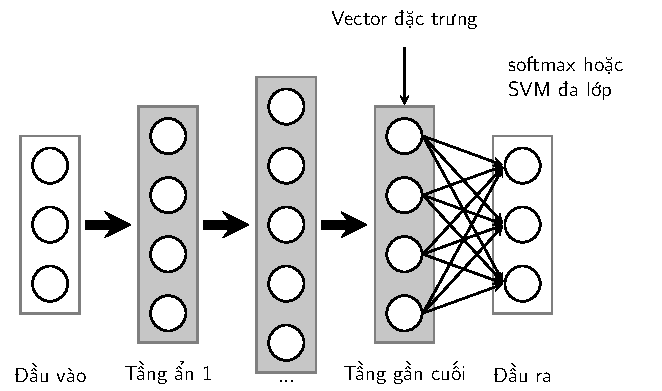
\includegraphics[width = \textwidth]{Chapters/01_Overview/q2_tl/latex/multi_layers.pdf}
    \caption[]{Kiến trúc deep learning cơ bản cho bài toán phân loại. Tầng cuối cùng là một tầng nối kín và thường là một hồi quy softmax.}
    \label{fig:transferlearning}
\end{figure}
%% ***************************************************************************** 
\index{tinh chỉnh -- fine-tuning}
Hướng tiếp cận thứ hai là sử dụng các mô hình đã được huấn luyện và cho huấn luyện thêm một vài tầng cuối dựa trên dữ liệu mới. Kỹ thuật này được
gọi là \textit{tinh chỉnh} ({fine-tuning}). {Việc này được thực hiện dựa trên quan
sát rằng những tầng đầu trong mạng neuron sâu trích xuất những đặc trưng chung mức thấp của đa số ảnh, các tầng cuối giúp trích chọn các đặc trưng mức cao phù hợp cho từng cơ sở dữ liệu (CSDL). Các đặc trưng mức cao có thể khác nhau tuỳ theo từng CSDL. Vì vậy, khi có dữ liệu mới, ta chỉ cần huấn luyện mạng neuron để trích chọn các đặc trưng mức cao phù hợp với dữ liệu mới này. 
 
Dựa trên kích thước và sự giống nhau giữa CSDL mới và CSDL gốc (dùng để huấn luyện mạng neuron ban đầu), có một vài quy tắc để huấn luyện mạng neuron mới\footnote{\textit{Transfer Learning, CS231n} (\url{https://goo.gl/VN1g7F})}: 

\begin{itemize}
\item \textit{CSDL mới nhỏ, tương tự CSDL gốc.} Vì CSDL mới nhỏ, việc
tiếp tục huấn luyện mô hình có thể dễ dẫn đến hiện tượng \textit{quá khớp} (overfitting, xem Chương~\ref{cha:overfitting}). Cũng vì hai CSDL tương tự nhau, ta dự đoán
rằng các đặc trưng mức cao của chúng tương tự nhau. Vì vậy, ta không cần
huấn luyện lại mạng neuron mà chỉ cần huấn luyện một bộ phân loại dựa trên các vector đặc trưng thu được. 
 
\item \textit{CSDL mới lớn, tương tự CSDL gốc.} Vì CSDL này lớn,
quá khớp ít xảy ra hơn, ta có thể huấn luyện mô hình thêm một
vài vòng lặp. Việc huấn luyện có thể được thực hiện trên toàn bộ hoặc chỉ một
vài tầng cuối.
 
\item \textit{CSDL mới nhỏ, rất khác CSDL gốc.} Vì CSDL này nhỏ, tốt
hơn hết là dùng các bộ phân loại đơn giản khác để tránh quá khớp. Nếu muốn sử
dụng mạng neuron cũ, ta cũng chỉ nên tinh chỉnh các tầng cuối của nó. Hoặc có thể coi đầu ra của một tầng ở giữa của mạng neuron là vector đặc
trưng rồi huấn luyện thêm một bộ phân loại.
 
\item \textit{CSDL mới lớn rất khác CSDL gốc.} Thực tế cho thấy, sử dụng
các mạng neuron sẵn có trên CSDL mới vẫn hữu ích. Trong trường hợp này, ta vẫn có
thể sử dụng các mạng neuron sẵn có như là điểm khởi tạo của mạng neuron mới, không nên
huấn luyện mạng neuron mới từ đầu.
\end{itemize}
 
Một điểm đáng chú ý là khi tiếp tục huấn luyện các mạng neuron này, ta chỉ
nên chọn tốc độ học nhỏ để các hệ số mới không đi quá xa so với các
hệ số đã được huấn luyện ở các mô hình trước.
 
 
 
 
 
% \section{Đọc thêm}
% [1] \href{http://docs.opencv.org/3.1.0/da/df5/tutorial_py_sift_intro.html}{Introduction to SIFT (Scale-Invariant Feature Transform) - OpenCV} 
 
% [2] \href{http://machinelearningcoban.comIntroduction to SURF (Speeded-Up Robust Features}{Introduction to SURF (Speeded-Up Robust Features) - OpenCV}) 
 
% [3] \href{http://www.learnopencv.com/histogram-of-oriented-gradients/}{Histogram of Oriented Gradients - OpenCV} 
 
% [4] \href{http://cs231n.github.io/transfer-learning/#tf}{Transfer Learning} 
 
% [5] \href{http://sebastianruder.com/transfer-learning/}{Transfer Learning - Machine Learning's Next Frontier} 
 
% [6] \href{https://www.analyticsvidhya.com/blog/2017/06/transfer-learning-the-art-of-fine-tuning-a-pre-trained-model/}{Transfer learning & The art of using Pre-trained Models in Deep Learning} 

\section{Chuẩn hoá vector đặc trưng}
% (Tham khảo \href{https://en.wikipedia.org/wiki/Feature_scaling}{Feature Scaling wiki}). 
 
Các điểm dữ liệu đôi khi được đo đạc bằng những đơn vị khác nhau, chẳng hạn mét
và feet. Đôi khi, hai thành phần của dữ liệu ban đầu chênh lệch nhau lớn, chẳng
hạn một thành phần có khoảng giá trị từ 0 đến 1000, thành phần kia chỉ có khoảng
giá trị từ 0 đến 1. Lúc này, chúng ta cần chuẩn hóa dữ liệu trước khi thực hiện
các bước tiếp theo.
 
\textit{Chú ý}: việc chuẩn hóa này chỉ được thực hiện khi vector dữ liệu đã có cùng chiều. 
 
Sau đây là một vài phương pháp chuẩn hóa thường dùng.

\index{chuyển khoảng giá trị -- rescaling}
\subsection{Chuyển khoảng giá trị}
Phương pháp đơn giản nhất là đưa tất cả các đặc trưng về cùng một khoảng, ví dụ $[0, 1]$ hoặc $[-1, 1]$. Để muốn đưa đặc trưng thứ
$i$ của một vector đặc trưng $\bx$ về khoảng $[0, 1]$, ta sử dụng công thức
\begin{equation*} 
x_i' = \frac{x_i - \min(x_i)}{\max(x_i) - \min(x_i)} 
\end{equation*} 
trong đó $x_i$ và $x_i'$ lần lượt là giá trị đặc trưng ban đầu và giá trị đặc
trưng sau khi được chuẩn hóa. $\min(x_i), \max(x_i)$ là giá trị nhỏ nhất và lớn
nhất của đặc trưng thứ $i$ xét trên toàn bộ dữ liệu huấn luyện.
 
 
\subsection{Chuẩn hoá theo phân phối chuẩn}
\index{chuẩn hoá theo phân phối chuẩn -- standardization}
Một phương pháp khác thường được sử dụng là đưa mỗi đặc trưng về dạng một
phân phối chuẩn có kỳ vọng là 0 và phương sai là 1. Công thức chuẩn hóa
là 
\begin{equation*} 
x_i' = \frac{x_i - \bar{x}_i}{\sigma_i} 
\end{equation*} 
với $\bar{x}_i, \sigma_i$ lần lượt là kỳ vọng và độ lệch chuẩn của đặc trưng đó
xét trên toàn bộ dữ liệu huấn luyện.
 
\subsection{Chuẩn hoá về cùng norm}
Một lựa chọn khác cũng được sử dụng rộng rãi là biến vector dữ liệu thành vector
có độ dài Euclid bằng một. Việc này có thể được thực hiện bằng cách chia mỗi
vector đặc trưng cho $\ell_2$ norm của nó:
\begin{equation*}
\mathbf{x}' = \frac{\mathbf{x}}{\|\mathbf{x}\|_2} 
\end{equation*} 
 
 
% \section{Đọc thêm}
% \begin{enumerate}
%     \item  G. Csurka \etal, \textit{Visual categorization with bags
%     of keypoints}. Workshop on statistical learning in computer vision, ECCV.
%     Vol. 1. No. 1-22. 2004~\cite{csurka2004visual}.
    
%     \item S. Lazebnik \etal, \textit{Beyond bags
%         of features: Spatial pyramid matching for recognizing natural scene
%         categories.}, CVPR 2006~\cite{lazebnik2006beyond}

%     \item \textit{Preprocessing data, scikit learn}
%     (\url{https://goo.gl/gkCuUp}). 

% \end{enumerate}

 
